\chapter{First-Generation Quantum-Astronomy Science Cases}
\label{chap:e25}

\begin{chapteropening}
Over the previous parts we assembled our tools one by one, like gathering gear: complex amplitude and phase (Chapter \ref{chap:e01}), bandwidth and coherence time (Chapter \ref{chap:e02}), Poisson and shot noise (Chapter \ref{chap:e03}), second-order coherence \(g^{(2)}\) and the Siegert relation (Chapter \ref{chap:e08}), intensity interferometry and the van Cittert--Zernike theorem (Chapter \ref{chap:e10}), from visibility to imaging (Chapter \ref{chap:e11}), quantum estimation and SPADE (Chapter \ref{chap:e12}), event tables and clocks (Chapter \ref{chap:e13}), error budgets (Chapter \ref{chap:e15}), all the way to treating the star as a quantum light source (Chapter \ref{chap:e17}) and stitching transients into multi-messenger events (Chapter \ref{chap:e20}). With the gear ready, it is time to take the field. This chapter answers a very practical question: \textbf{under today's instrumental conditions, which pieces of ``doable right now'' real science can first-generation quantum astronomy actually do?} We walk down a checklist (bright-star angular diameters, the flattened spheroids of rapid rotators, close binaries, Be-star disks and Wolf--Rayet winds, the expansion of novae and Type Ia supernovae, the photon statistics of the Crab, natural-laser candidates), and at each stop we ask the same three things: \textbf{which observable do we measure? What array, exposure, and precision are needed? Which astrophysical question does it answer?} This is not pie in the sky but the mapping of every formula from the previous chapters onto targets you could point at tomorrow night.
\end{chapteropening}

\section{Ranking the cases: three yardsticks: brightness, angular scale, external priors}
\label{sec:e25-triage}

You cannot fight a battle by charging in all at once. What a first-generation project fears most is not ``the topic is not pretty enough'' but ``a pretty topic that yields no result.'' So before picking targets, one must establish a cool-headed ranking method, letting scientific value, technical feasibility, and residual product-after-failure all enter the judgment at once.

\textbf{The first yardstick is brightness.} The signal of intensity interferometry is the coincidence count, and its statistical precision is ultimately set by the \textbf{number of photon pairs} accumulated (Chapter \ref{chap:e15}). The higher the photon rate, the more pairs gathered in the same time, and the error falls as the square root of the pair count. For the present generation of instruments, a rough zoning is: hot stars with visual magnitude \(m_V\lesssim5\) are the ``verification zone,'' with strong signals that can be reproduced repeatedly; \(m_V\simeq6\text{--}7\) is the ``challenging but plannable'' zone; and \(m_V\gtrsim9\) usually requires larger arrays, multiple spectral channels, longer integration, or lower system noise to reach. The estimate of LeBohec and Holder gives a memorable anchor: a pair of \(100\,\mathrm{m^2}\) telescopes with electronic bandwidth at the GHz level can, within 5 hours, achieve a several-sigma correlation detection on a source of \(m_V\simeq6.7\) \citep{2006ApJ...649..399L,2013APh....43..331D}.

\textbf{The second yardstick is angular scale.} Brightness decides ``whether there are photons''; angular scale decides ``whether these photons can become parameters.'' As Chapter \ref{chap:e11} explained, an interferometer with baseline \(B\) and wavelength \(\lambda\) can resolve angular scales down to \(\lambda/B\). If the target angular scale \(\theta\gg\lambda/B\), then on long baselines the squared visibility \(|V|^2\) has already fallen nearly to zero, and only short baselines retain signal; if \(\theta\ll\lambda/B\), then all baselines see an ``unresolved point,'' the derivative of the visibility with respect to diameter is nearly zero, and measuring it constrains the parameters hardly at all. Both extremes are bad; the most comfortable case is to have the main structure fall right within the range of baselines you have: \(50\text{--}300\,\mathrm{m}\) for existing IACT arrays, and \(0.5\text{--}2\,\mathrm{km}\) for future CTA-type arrays.

\textbf{The third yardstick is external priors.} The same few \(|V|^2\) data points, if you know in advance the distance, spectrum, orbit, radial velocity, or a theoretical atmosphere model, can be ``translated'' into real physical parameters; if you have no prior at all, a few isolated visibility points are often mutually degenerate, and none can pin down another. So targets with mature priors naturally rank ahead \citep{2003RPPh...66..789M,2012MNRAS.419..172N}.

Writing these three yardsticks into a scorable ranking expression yields a practical triage tool:
\begin{equation}
  \mathcal P
  =
  \frac{
  W_{\rm sci}\,
  R_{\rm tech}\,
  R_{\rm prior}
  }{
  1+R_{\rm sys}+R_{\rm trigger}
  } .
  \label{eq:e25-priority-score}
\end{equation}
\begin{formulaexplain}
\(\mathcal P\) is the project ranking score. In the numerator, the higher the science return \(W_{\rm sci}\), the technical maturity \(R_{\rm tech}\), and the external prior \(R_{\rm prior}\), the higher the score; in the denominator, the higher the systematic-error risk \(R_{\rm sys}\) and the trigger/scheduling risk \(R_{\rm trigger}\), the lower the score. It is designed specifically to prevent starting a project ``just because the topic sounds nice.''
\end{formulaexplain}
Grounding each term: \(W_{\rm sci}\) is the science return (how important this result is), \(R_{\rm tech}\) is the technical maturity (whether existing instruments can stably deliver it), \(R_{\rm prior}\) is the external prior and model interpretability, \(R_{\rm sys}\) is the systematic-error risk (how easily zero-baseline correlation, time synchronization, and background subtraction go wrong), and \(R_{\rm trigger}\) is the trigger and scheduling risk (whether one must compete for a time window, and whether one can start up at any time). These quantities are all dimensionless; in practice one need only grade them coarsely (high/medium/low), the aim being not to compute a precise decimal but to \textbf{prevent any single dimension from dominating the choice}. A comparison: the geometric distance of Type Ia has extremely high \(W_{\rm sci}\), but its \(R_{\rm trigger}\) and \(R_{\rm sys}\) are also high, propping up the denominator, so the first generation should not force it; the angular diameter of bright stars has only moderate \(W_{\rm sci}\), yet very high \(R_{\rm tech}\) and very low system risk, so its score is instead steady, making it especially suitable as one of the first batch of ``acceptance metrics'' \citep{2024ApJ...966...28A,2024MNRAS.529.4387A,2025PhRvD.111h3047K}.

\begin{figure}[tbp]
\centering
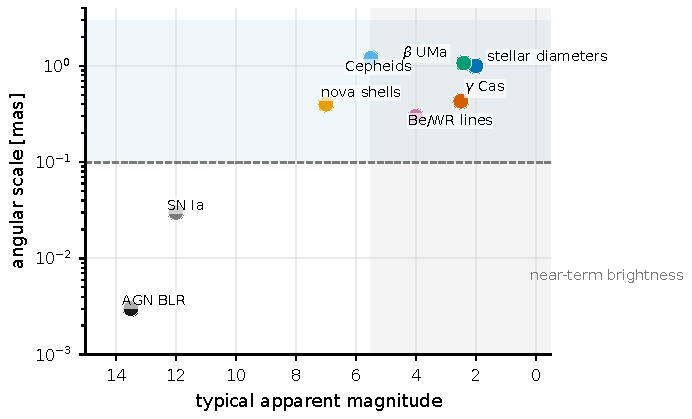
\includegraphics[width=0.88\linewidth]{figures/generated/chapter_19/ch19_science_case_feasibility.pdf}
\caption{The positions of first-generation candidate targets on the ``brightness--angular scale'' plane. Bright-star angular diameters, \(\beta\) UMa, \(\gamma\) Cas, and the Be/WR spectral-line regions simultaneously satisfy ``bright enough'' and ``resolvable by hundred-meter baselines,'' falling in the most comfortable region; Type Ia, AGN broad-line regions, and dark-matter small-scale lensing have very high scientific value, yet are pushed toward long-term projects by brightness, event rate, or angular scale. This figure is the visualization of the three yardsticks in Eq.\ \eqref{eq:e25-priority-score}.}
\label{fig:e25-case-plane}
\end{figure}

With this ranking in hand, the order of the rest of this chapter is in fact already implicit: first do the targets that fall in the upper-right ``comfortable region'' of Figure \ref{fig:e25-case-plane}, then step by step push toward directions of higher scientific value but also higher risk.

\section{Stellar angular diameter and effective temperature: the most mature first-generation product}
\label{sec:e25-diameter}

Why is the first task to measure a star's \textbf{angular diameter}? Because it simultaneously satisfies the three yardsticks above, and its output is direct, reproducible, and can serve repeatedly as an acceptance standard. The observable is very clean: measure the squared visibility \(|V|^2(B,\lambda)\) over a range of baselines \(B\) and wavelengths \(\lambda\), and the model begins from the simplest \textbf{uniform disk}, then corrects with a \textbf{limb-darkening} (the disk's edge is dimmer than its center) profile or a full atmosphere model.

The most elegant use of angular diameter is that it directly pins down a star's \textbf{effective temperature}. Not a single step in this chain of logic can be skipped, so we lay it out. A star of radius \(R\) and effective temperature \(T_{\rm eff}\) has luminosity given by the Stefan--Boltzmann law, \(L=4\pi R^2\sigma_{\rm SB}T_{\rm eff}^4\). These photons travel to the Earth at distance \(D\), spread over a sphere of radius \(D\), so the \textbf{bolometric flux} we receive is
\[
  F_{\rm bol}=\frac{L}{4\pi D^2}
  =\frac{R^2}{D^2}\,\sigma_{\rm SB}T_{\rm eff}^4
  =\left(\frac{R}{D}\right)^2\sigma_{\rm SB}T_{\rm eff}^4 .
\]
Note that \(R/D\) is precisely the star's \textbf{angular radius}, and the angular diameter \(\theta_{\rm LD}=2R/D\), so \(R/D=\theta_{\rm LD}/2\) and \((R/D)^2=\theta_{\rm LD}^2/4\). Substituting back gives the central equation of this section:
\begin{equation}
  F_{\rm bol}
  =
  \frac{\theta_{\rm LD}^2}{4}
  \sigma_{\rm SB}T_{\rm eff}^4,
  \qquad
  T_{\rm eff}
  =
  \left(
  \frac{4F_{\rm bol}}
  {\sigma_{\rm SB}\theta_{\rm LD}^2}
  \right)^{1/4}.
  \label{eq:e25-teff}
\end{equation}
\begin{formulaexplain}
\(F_{\rm bol}\) is the bolometric flux received at Earth, \(\theta_{\rm LD}\) is the limb-darkened angular diameter, \(\sigma_{\rm SB}\) is the Stefan--Boltzmann constant, and \(T_{\rm eff}\) is the effective temperature. In a word: once the angular diameter is measured accurately, ``flux'' can be directly converted into the star's ``temperature scale.''
\end{formulaexplain}
Accounting for units and dimensions one by one: \(F_{\rm bol}\) has units \(\mathrm{erg\,s^{-1}\,cm^{-2}}\), obtained by integrating multiband photometry; \(\theta_{\rm LD}\) has units of rad (the milliarcsecond, mas, is a common practical unit, with \(1\,\mathrm{mas}=4.85\times10^{-9}\,\mathrm{rad}\)); \(\sigma_{\rm SB}=5.67\times10^{-5}\,\mathrm{erg\,s^{-1}\,cm^{-2}\,K^{-4}}\); and \(T_{\rm eff}\) has units of K. The beauty of this equation is that it is \textbf{independent of distance}: both \(F_{\rm bol}\) and \(\theta_{\rm LD}\) are directly observable, and the intervening \(D\) has already canceled out in the derivation.

How does the error in angular diameter propagate to the temperature? Take the logarithmic differential of \(T_{\rm eff}\) with respect to \(\theta_{\rm LD}\). Because \(T_{\rm eff}\propto\theta_{\rm LD}^{-1/2}\) (treating \(F_{\rm bol}\) as an independent measurement), we have
\[
  \ln T_{\rm eff}=\text{const}-\tfrac12\ln\theta_{\rm LD}
  \;\Longrightarrow\;
  \frac{\delta T_{\rm eff}}{T_{\rm eff}}=-\frac12\frac{\delta\theta_{\rm LD}}{\theta_{\rm LD}} .
\]
So a \(4\%\) error in angular diameter, propagated by this path alone, becomes only \(2\%\) in temperature. This ``halving'' relation explains why bright-star angular diameters are worth measuring again and again: it is not a one-off instrumental flourish but \textbf{foundational data} that flows into \(T_{\rm eff}\), stellar radius, age, rotation models, and the standard-star scale \citep{1967MNRAS.137..393H,1977MNRAS.180..177B,2003RPPh...66..789M}.

This route has traveled from history into the present. Last century the Narrabri intensity interferometer measured the diameters of a batch of bright stars using the method of Hanbury Brown and Twiss \citep{1956Natur.178.1046H,1974MNRAS.167..121H}; today VERITAS's intensity-interferometry system (VERITAS-SII) has advanced it to sub-milliarcsecond precision, giving diameters for \(\beta\) CMa and \(\epsilon\) Ori, and achieving better than \(5\%\) with far less observing time than in the old days; a subsequent measurement of \(\beta\) UMa at 416 nm gave a limb-darkened angular diameter \(\theta_{\rm LD}=1.07\pm0.04_{\rm stat}\pm0.05_{\rm sys}\,\mathrm{mas}\), cross-checked against CHARA near-infrared and Keck mid-infrared results. MAGIC's upgraded system (MAGIC-SII) reported 22 stellar diameters in one go, 13 of them with no prior comparable measurement: intensity interferometry has gone from ``a single demonstration'' to ``producing data in batches'' \citep{2020NatAs...4.1164A,2024ApJ...966...28A,2024MNRAS.529.4387A}. One point to note here is that these results use \textbf{second-order} coherence (Chapters \ref{chap:e08}, \ref{chap:e10}), which is insensitive to atmospheric seeing and optical-path phase, and this is precisely why it can still work on narrowband, ultra-long baselines.

\textbf{What is needed, what is answered?} The array this case needs is very plain: a few pairs of off-the-shelf IACT telescopes, hundred-meter baselines, narrowband filtering, GHz-level electronic bandwidth, and integration from a few hours to a few nights; the precision goal is to measure the diameter to \(3\text{--}5\%\), reproducible over multiple nights. It answers the most basic question in stellar physics, \textbf{just how big and how hot this star really is}, and thereby calibrates the entire scale of stellar parameters and distances.

\section{Rapid rotation: upgrading from ``how big'' to ``what shape''}
\label{sec:e25-rotation}

Measuring the diameter is only the first step. Many hot stars rotate so fast that centrifugal force flings the equator into a bulge, and the photosphere becomes a flattened ellipsoid; moreover, by the von Zeipel theorem, the bulging equator has weaker gravity, lower temperature, and is dimmer, while the poles are brighter and hotter; this is \textbf{gravity darkening}. To see such structure, the uniform-disk model no longer suffices: it has only one parameter \(\theta\), whereas a flattened ellipsoid needs at least three: the minor-axis angular diameter \(\theta_{\rm min}\), the \textbf{axial ratio} \(r=\theta_{\rm maj}/\theta_{\rm min}\), and the position angle \(\varphi_\star\).

How do we write this flattened sphere as a fittable visibility curve? First recall the known result of Chapter \ref{chap:e11}: a uniform disk of angular diameter \(\theta\) has first-order visibility modulus of Airy form \(|V|=|2J_1(x)/x|\), where \(x=\pi B\theta/\lambda\) is the dimensionless spatial frequency and \(J_1\) is the first-order Bessel function (the standard result for circular-aperture diffraction, with its first zero at argument \(3.83\)). The trick for the ellipsoid is that the ``effective diameter'' seen along different projection directions differs: seen along the minor axis it is \(\theta_{\rm min}\), and seen along the major axis it is \(r\theta_{\rm min}\). Folding this directional dependence into \(x\) gives
\begin{equation}
  x_{\rm ell}
  =
  \frac{\pi B_p\theta_{\rm min}}{\lambda}
  \left[
  \cos^2\psi
  +
  r^2\sin^2\psi
  \right]^{1/2},
  \qquad
  |V_{\rm ell}|^2
  =
  \left[\frac{2J_1(x_{\rm ell})}{x_{\rm ell}}\right]^2 .
  \label{eq:e25-elliptical-visibility}
\end{equation}
\begin{formulaexplain}
\(x_{\rm ell}\) is the dimensionless spatial frequency of the flattened ellipsoid on the current projected baseline, \(B_p\) is the projected baseline length, \(\psi\) is the direction angle of the projected baseline relative to the minor axis, and \(r\) is the axial ratio. The factor in the brackets folds ``the direction of viewing'' into the effective diameter: along the minor axis (\(\psi=0\)) it reduces to \(\theta_{\rm min}\), and along the major axis (\(\psi=90^\circ\)) it becomes \(r\theta_{\rm min}\).
\end{formulaexplain}
Check the bracket once and its geometry is clear: when \(\psi=0\) (baseline aligned with the minor axis), \(\cos^2\psi=1,\sin^2\psi=0\), so \(x_{\rm ell}=\pi B_p\theta_{\rm min}/\lambda\), and one sees the minor axis; when \(\psi=90^\circ\), \(x_{\rm ell}=\pi B_p(r\theta_{\rm min})/\lambda\), and one sees the major axis. Grounding the parameters: hot-star axial ratios are typically \(r\simeq1.1\text{--}1.5\), with minor-axis angular diameters often below \(1\,\mathrm{mas}\). Here is a key \textbf{observation-design} lesson: to pin down both \(r\) and \(\varphi_\star\) at once, you must obtain \(|V|^2\) at \textbf{multiple position angles}: single-direction baseline coverage badly degenerates \(r\) and \(\varphi_\star\), because one curve can be jointly fit by ``more flattened but rotated'' and ``less flattened.'' This is precisely the language of uv coverage from Chapter \ref{chap:e11} cashed out on a concrete target.

In reality this has already been done. VERITAS's observation of the classic rapid rotator \(\gamma\) Cas gave a minor-axis angular diameter of about \(0.43\pm0.02_{\rm stat}\pm0.02_{\rm sys}\,\mathrm{mas}\), an axial ratio of about \(1.28\pm0.04\pm0.02\), and a rotation-axis position angle of about \(116^\circ\), and inferred with a Roche--von Zeipel model that it is already near \textbf{critical (breakup) rotation}, where the equatorial centrifugal force nearly balances gravity \citep{2025ApJ...995..191A}. This means first-generation intensity interferometry can already advance from ``how big is this star'' to ``what shape is this star, and how much do the poles and equator differ in temperature.''

\textbf{What is needed, what is answered?} This case needs coverage of \textbf{two or more distinctly different position angles} on the same target, with all other requirements the same as for angular diameter; the precision goal is to statistically distinguish the disk model from the ellipse model. It answers a deep question in stellar structure and evolution: \textbf{how rotation alters a star's shape, temperature distribution, and even lifetime}.

\section{Binaries, Be-star disks, and Wolf--Rayet winds: separating them with the baseline}
\label{sec:e25-binary}

Intensity interferometry can measure not only ``how big a source is'' but also see through ``it is actually two sources.'' The advantage of a \textbf{close binary} is that its signal has an extremely high recognizability. Consider two unresolved point sources with angular separation vector \(\bm s\) and \textbf{flux ratio} \(f=F_2/F_1\). Their combined coherence function is the superposition of the individual complex amplitudes weighted by flux; after normalization it is \((1+f\,e^{-2\pi i\,\bm u\cdot\bm s})/(1+f)\), where \(\bm u=\bm B_\perp/\lambda\) is the spatial frequency. The squared visibility is its modulus squared, and we expand this step without skipping any:
\[
  |V_{\rm binary}|^2
  =\frac{|1+f e^{-i\phi}|^2}{(1+f)^2},
  \qquad \phi\equiv 2\pi\,\bm u\cdot\bm s .
\]
Using \(|1+f e^{-i\phi}|^2=(1+f\cos\phi)^2+(f\sin\phi)^2=1+2f\cos\phi+f^2\cos^2\phi+f^2\sin^2\phi=1+f^2+2f\cos\phi\) (using only \(\cos^2+\sin^2=1\)), we obtain
\begin{equation}
  |V_{\rm binary}|^2
  =
  \frac{1+f^2+2f\cos(2\pi\,\bm u\cdot\bm s)}
  {(1+f)^2}.
  \label{eq:e25-binary-visibility}
\end{equation}
\begin{formulaexplain}
\(\bm u=\bm B_\perp/\lambda\) is the spatial frequency, \(\bm s\) is the binary angular-separation vector, and \(f\) is the flux ratio. The phase in the exponent varies with the baseline, making \(|V|^2\) \textbf{oscillate} along the baseline: it is precisely this oscillating curve that lets intensity interferometry constrain the separation and orientation of the binary.
\end{formulaexplain}
The key to reading this equation is the \textbf{amplitude} of that cosine term, \(2f/(1+f)^2\). When \(f=1\) (equal-brightness binary), \(|V|^2\) oscillates all the way from \(1\) (at \(\cos=+1\)) to \(0\) (at \(\cos=-1\)), a deep and easily recognizable signal; when \(f=0.1\) (a faint companion only one-tenth as bright as the primary), the half-amplitude of the cosine term is only \(2(0.1)/(1.1)^2\simeq0.17\), and \(|V|^2\) swings by this half-amplitude about its mean \((1+f^2)/(1+f)^2=1.01/1.21\simeq0.83\), that is, it ripples from a trough of \((1-f)^2/(1+f)^2=(0.9/1.1)^2\simeq0.67\) to a peak of \(1.0\), a modulation depth of only about \(0.33\), sharply raising the demands on signal-to-noise and calibration. The \textbf{period} of the oscillation is set by the separation \(\bm s\): the larger the separation, the faster \(|V|^2\) oscillates with baseline. So binary projects are best suited to systems that \textbf{already have spectroscopic-orbit or eclipsing-binary priors}: each night one need only obtain a few baseline points to be threaded onto a known orbit model; even if a given night fails, one can still give an upper limit on the separation or brightness ratio, so the night is not a total loss \citep{1974MNRAS.167..121H,2012MNRAS.419..172N,2014MNRAS.437..798M,2022MNRAS.512.1722K}.

\begin{figure}[tbp]
\centering
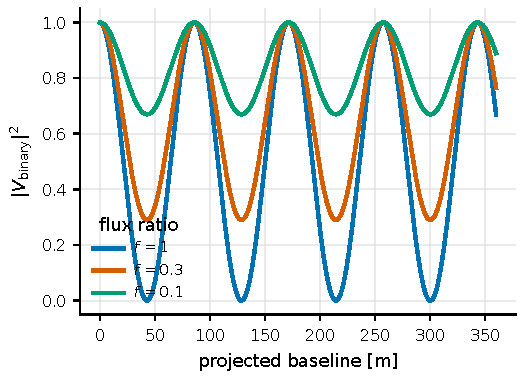
\includegraphics[width=0.82\linewidth]{figures/generated/chapter_19/ch19_binary_visibility.pdf}
\caption{The squared-visibility oscillation of a \(1\,\mathrm{mas}\) binary at 416 nm. An equal-brightness binary (\(f=1\)) gives a deep oscillation from 1 to 0; as the flux ratio drops to \(0.3\) then \(0.1\), it rapidly shallows following the amplitude \(2f/(1+f)^2\) of Eq.\ \eqref{eq:e25-binary-visibility}. Binary projects therefore depend especially on multi-position-angle baseline coverage and known orbital priors; otherwise the brightness ratio, separation, and position angle become mutually degenerate.}
\label{fig:e25-binary-visibility}
\end{figure}

One step further is to combine ``spatial resolution'' with ``spectral-line selection'' to dissect \textbf{Be-star decretion disks} (equatorial gas disks thrown off by rapidly rotating B-type stars) and \textbf{Wolf--Rayet winds} (high-speed stellar winds of massive stars). The continuum of these sources comes mainly from the photosphere, while emission lines such as \(\mathrm{H}\alpha\), He, and Fe come from a larger, more extended disk or wind-collision region. The trouble is that within a single filter the \textbf{line and continuum are often mixed}, and the measured visibility is a flux-weighted average of the two:
\begin{equation}
  V_{\rm obs}
  =
  \frac{
  F_{\rm c}V_{\rm c}
  +
  F_{\rm line}V_{\rm line}
  }{
  F_{\rm c}+F_{\rm line}
  } .
  \label{eq:e25-line-continuum}
\end{equation}
\begin{formulaexplain}
\(V_{\rm c},V_{\rm line}\) are respectively the visibilities of the continuum region and the line region, and \(F_{\rm c},F_{\rm line}\) are the corresponding fluxes. The \(V_{\rm obs}\) you measure is a flux-weighted average of the two, so the line geometry must first be ``subtracted'' from the continuum before it can be interpreted on its own.
\end{formulaexplain}
Here \(F_{\rm line}/F_{\rm c}\) can be estimated from simultaneous spectroscopy or a ``narrowband-minus-continuum'' dual-filter measurement. The physical reading is intuitive: if the line region is \textbf{larger} than the photosphere (as for an extended disk), then \(V_{\rm line}\) falls faster than the continuum on long baselines, and the mixed \(V_{\rm obs}\) is pulled down by the line at the long-baseline end; conversely, if the line comes from a very small, high-brightness spot, it instead retains signal on long baselines. Historically the Narrabri measurement of the Wolf--Rayet binary \(\gamma^2\) Velorum already showed that the emission-line region and the continuum region can have \textbf{different angular scales} \citep{1970MNRAS.148..103H,2010SPIE.7734E..0AD,2012NewAR..56..143D,2025ApJ...995..191A}. Modern multi-baseline arrays can generalize this idea to the geometry of Be-star disks, the line profiles of rapidly rotating hot stars, and the wind-collision regions of interacting binaries.

\textbf{What is needed, what is answered?} This case needs narrowband filtering or simultaneous spectroscopy to separate line from continuum, a verifiable continuum subtraction, and sufficient line flux; it answers questions like \textbf{how a star ejects matter, and what geometry the disk and wind take}, questions hard to image directly by other means.

\section{Expanding transients: novae are doable now, Type Ia is a long-term goal}
\label{sec:e25-transient}

Now turn the lens to sources that ``grow.'' Novae and supernovae eject an expanding shell whose geometric ledger is extremely simple: if the shell expands approximately freely at velocity \(v_{\rm exp}\), then at time \(t-t_0\) after the outburst, the angular diameter it subtends is ``twice the traversed linear radius divided by the distance'':
\begin{equation}
  \theta(t)
  \simeq
  \frac{2v_{\rm exp}(t-t_0)}{D},
  \qquad
  D
  \simeq
  \frac{2v_{\rm exp}(t-t_0)}{\theta}.
  \label{eq:e25-expansion}
\end{equation}
\begin{formulaexplain}
\(\theta(t)\) is the angular diameter of the expanding shell, \(v_{\rm exp}\) is the expansion velocity, \(t_0\) is the outburst time, and \(D\) is the distance. The left equation predicts ``how big the shell is,'' and the right inverts it for ``how far away we are'': this is the \textbf{expansion parallax}, independent of a standard candle.
\end{formulaexplain}
Accounting term by term: \(v_{\rm exp}\) comes from the Doppler velocity of spectral lines (Chapter \ref{chap:e20} explained how to read velocity from wavelength shifts), with units \(\mathrm{cm\,s^{-1}}\); \(t-t_0\) is the time after outburst, with units s; and \(D\) is the distance, with units cm. Its physical premise is a plain statement: \(v_{\rm exp}\) and \(\theta\) must correspond to \textbf{the same layer of matter}, otherwise the distance from the right equation is systematically biased (Chapter \ref{chap:e20} analyzed this trap in detail).

Substituting two sets of real numbers, what the first generation can and cannot do becomes immediately clear. \textbf{Galactic nova}: take \(D=2\,\mathrm{kpc}=6.17\times10^{21}\,\mathrm{cm}\), \(v_{\rm exp}=10^8\,\mathrm{cm\,s^{-1}}\), \(t-t_0=10\,\mathrm{d}=8.64\times10^5\,\mathrm{s}\). The linear radius \(v_{\rm exp}(t-t_0)=8.64\times10^{13}\,\mathrm{cm}\), and the angular diameter \(\theta=\dfrac{2\times8.64\times10^{13}}{6.17\times10^{21}}=2.80\times10^{-8}\,\mathrm{rad}\). Converting with \(1\,\mathrm{rad}=2.063\times10^8\,\mathrm{mas}\), \(\theta\approx5.8\,\mathrm{mas}\), within ten days it reaches a few milliarcseconds, resolvable with baselines below one hundred meters. \textbf{Type Ia supernova}: take \(D=10\,\mathrm{Mpc}=3.09\times10^{25}\,\mathrm{cm}\), \(v_{\rm exp}=10^9\,\mathrm{cm\,s^{-1}}\), \(t-t_0=20\,\mathrm{d}=1.73\times10^6\,\mathrm{s}\). The linear radius \(1.73\times10^{15}\,\mathrm{cm}\), and \(\theta=\dfrac{2\times1.73\times10^{15}}{3.09\times10^{25}}=1.12\times10^{-10}\,\mathrm{rad}\approx0.023\,\mathrm{mas}\), even with a velocity ten times higher, twenty days later it is only a few tens of microarcseconds, needing \textbf{kilometer-scale} optical baselines to reach.

\begin{figure}[tbp]
\centering
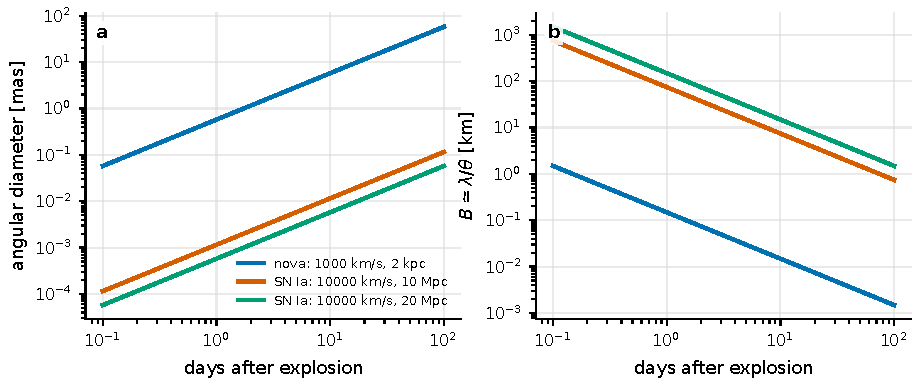
\includegraphics[width=0.94\linewidth]{figures/generated/chapter_19/ch19_transient_expansion.pdf}
\caption{The angular diameter of expanding transients and the required baseline. A Galactic nova enters the milliarcsecond regime within a few days to a few tens of days, well suited for the first generation to rehearse the whole ``trigger--schedule--image'' chain; a Type Ia at \(10\text{--}20\,\mathrm{Mpc}\) is only a few tens of microarcseconds even near peak, requiring kilometer-scale baselines and a nearby event with \(m\lesssim12\). The curves are precisely the behavior of Eq.\ \eqref{eq:e25-expansion} for various \(v_{\rm exp}\) and \(D\).}
\label{fig:e25-transient-expansion}
\end{figure}

So the first generation's division of labor is clear: the \textbf{Galactic nova} is a realistic target, its angular scale large enough and bright enough, best suited for running through the whole pipeline of trigger, filtering, background subtraction, and model fitting, with the main difficulties coming from rapid brightness evolution, non-spherical shell asymmetry, and dust obscuration. The \textbf{geometric distance of Type Ia} is a high-return long-term goal: the feasibility study of Kim et al.\ takes \(m\lesssim12\) (corresponding to a local volume of \(z\sim0.004\), about one per year over the whole sky) as the brightness range foreseeable for the next generation, and uses radiative-transfer models to compute the surface brightness and \(|V|^2\) at various wavelengths, pointing out that \textbf{spectral resolution} can provide multiwavelength tomography, so the measurement is no longer confined to a single uniform-disk radius \citep{2025PhRvD.111h3047K,1997A&A...320..799F,2004A&A...415..531S}. In other words, the Type Ia distance ruler should be slotted into second-generation or dedicated arrays, not into the first generation's acceptance items.

\textbf{What is needed, what is answered?} The nova case needs \textbf{fast triggering} (responding within hours) plus simultaneous line velocities, pairing \(\theta(t)\) with \(v_{\rm exp}\); it answers ``how far away this outburst is, and whether the shell is spherically symmetric,'' and lays technical groundwork for future use of expansion parallax to independently calibrate the cosmic distance ladder.

\section{The Crab and natural lasers: testing ``non-thermal'' with photon statistics}
\label{sec:e25-statistics}

The previous sections all used \textbf{visibility} (the spatial information of second-order coherence). This section switches glasses to \textbf{temporal statistics}: precisely where the event table (Chapter \ref{chap:e13}) and \(g^{(2)}\) (Chapter \ref{chap:e08}) come into their own.

First the \textbf{Crab pulsar}. It is not a good target for spatial intensity interferometry (it is a point source), but it is an excellent object for event-table science: bright, stably periodic, with a precise ephemeris, and an optical main pulse and interpulse that define clear \textbf{phase windows}. The premise for placing each photon into the correct phase window is that the time stamp is accurate enough. The conversion between phase error and time error is a single line:
\begin{equation}
  \Delta\phi
  =
  \frac{\Delta t}{P_{\rm spin}}.
  \label{eq:e25-pulse-phase}
\end{equation}
\begin{formulaexplain}
\(\Delta t\) is the photon time-stamp error, \(P_{\rm spin}\) is the pulsar spin period, and \(\Delta\phi\) is the converted phase error (dimensionless, with \(0\text{--}1\) corresponding to a full period). The more accurate the timing, the better the photon can be placed into the pulse-phase window it truly belongs to.
\end{formulaexplain}
Order of magnitude: the Crab's \(P_{\rm spin}\simeq33\,\mathrm{ms}\), and a \(1\,\mu\mathrm{s}\) timing error corresponds to only \(\Delta\phi\simeq10^{-6}/(33\times10^{-3})\approx3\times10^{-5}\); extremely comfortable, microsecond-level synchronization is ample. But the same equation tells you that a millisecond pulsar (\(P\sim\mathrm{ms}\)), to preserve the same narrow phase structure, must push \(\Delta t\) down to the nanosecond level. With phase windows in hand, one can do what past average light curves could not: phase-resolved \(g^{(2)}\), color correlations, and conditional stacking against radio \textbf{giant pulses}. Instruments like AquEYE/Iqueye can already save photons with picosecond-to-nanosecond time tags; observationally, the optical emission is enhanced in periods with Crab giant radio pulses, and ARCONS also saw that earlier-arriving giant pulses correspond to stronger optical enhancement \citep{2009JMOp...56..261B,2009A&A...508..531N,2015SPIE.9504E..0CZ,2003Sci...301..493S,2013ApJ...779L..12S}. What first-generation quantum astronomy is to do is upgrade these results from ``average light curves'' to ``event-table statistics + polarization/color windowing.''

\begin{figure}[tbp]
\centering
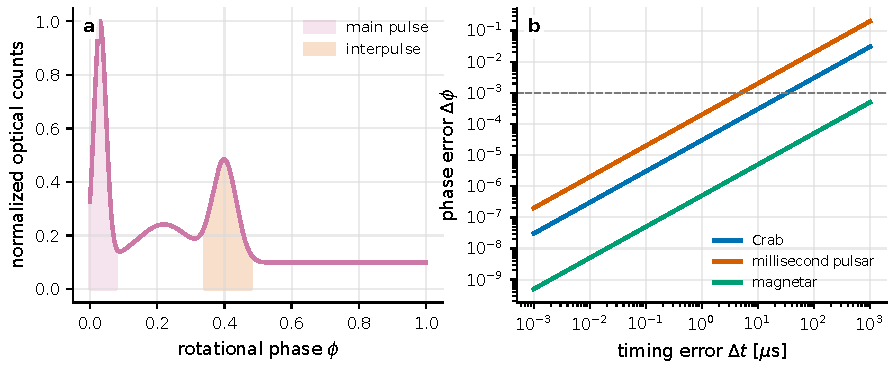
\includegraphics[width=0.94\linewidth]{figures/generated/chapter_19/ch19_crab_phase_windows.pdf}
\caption{The phase windows and time error of Crab-type optical pulses. The left panel sketches the three event-selection windows of main pulse, bridge, and interpulse; the right panel converts the time error into phase error via Eq.\ \eqref{eq:e25-pulse-phase}. For the Crab, microsecond-level timing is more than enough; for millisecond pulsars, ns--\(\mu\mathrm{s}\)-level synchronization is needed to preserve the narrow phase structure.}
\label{fig:e25-crab-phase}
\end{figure}

Next, \textbf{natural-laser} (natural / astrophysical laser) candidates. What these targets test is a very pure quantum question: \textbf{are the photon statistics of this bright spectral line thermal or coherent?} But beware a trap: ``seeing a bright spectral line'' is by itself \textbf{insufficient} to declare a laser, because the superposition of many mutually incoherent thermal modes can also average away the bunching peak. Quantitatively, for \(M\) mutually incoherent thermal modes,
\begin{equation}
  g^{(2)}(0)-1
  =
  \frac{1}{M},
  \label{eq:e25-mode-bunching}
\end{equation}
\begin{formulaexplain}
\(M\) is the number of mutually incoherent thermal modes superposed in the detection, and \(g^{(2)}(0)\) is the zero-delay second-order coherence. Single-mode thermal light has \(g^{(2)}(0)=2\) (bunching), but the larger \(M\), the more the bunching peak is averaged away, and \(g^{(2)}(0)\to1\). So \(g^{(2)}(0)\) close to 1 does not necessarily mean the light is an ideal laser.
\end{formulaexplain}
For comparison, remember the two extremes of Chapter \ref{chap:e08}: single-mode thermal state \(g^{(2)}(0)=2\), and ideal coherent state \(g^{(2)}(0)=1\). Equation \eqref{eq:e25-mode-bunching} says that ``multimode thermal light disguises itself as coherent light,'' so this kind of test must be accompanied by a \textbf{null test}: accounting cleanly for the mode number, the instrument time response, and the continuum background, before one can judge what a deviation of \(g^{(2)}(0)\) from 1, or its proximity to 1, means. Another usable handle is the line width: if the line width is \(\Delta\nu\), the coherence time is about \(\tau_c\sim1/(\pi\Delta\nu)\) (the concrete form of the bandwidth--coherence-time relation of Chapter \ref{chap:e02}). For example, if a natural-laser line is as narrow as \(\Delta\nu\sim1\,\mathrm{GHz}\), then \(\tau_c\sim1/(\pi\times10^9)\approx3\times10^{-10}\,\mathrm{s}=0.3\,\mathrm{ns}\); the narrower the line and the longer the coherence time, the easier it is to preserve a resolvable correlation \textbf{contrast} at a given detector time resolution. Among real candidates, the Fe II lines in the Weigelt blobs of Eta Carinae are pumped by \(\mathrm{Ly}\alpha\), and Johansson and Letokhov discussed Fe II laser lines at \(0.9\text{--}1.0\,\mu\mathrm{m}\) and in the near-infrared; line-width measurement plus photon-correlation spectroscopy can provide direct evidence \citep{2004A&A...428..497J,2005NewA...10..361J,2008AIPC..984..216D}.

\begin{figure}[tbp]
\centering
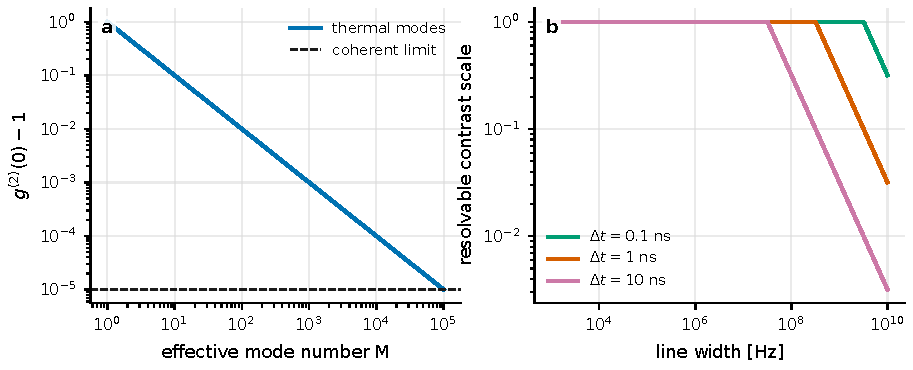
\includegraphics[width=0.94\linewidth]{figures/generated/chapter_19/ch19_natural_laser_statistics.pdf}
\caption{Two statistical criteria for natural-laser candidates. The left panel shows that increasing the number of thermal modes \(M\) lowers the bunching peak per Eq.\ \eqref{eq:e25-mode-bunching}, approaching the coherent limit \(g^{(2)}(0)-1=0\); the right panel shows that the narrower the line and the longer the coherence time, the easier it is to preserve a resolvable contrast at a given time resolution. Together they show: judging ``whether it is a laser'' requires jointly using photon statistics and line width, with a rigorous null test.}
\label{fig:e25-natural-laser}
\end{figure}

\textbf{What is needed, what is answered?} These two classes of case depend more on \textbf{event-table quality}: absolute time synchronization, a precise ephemeris, a verifiable background subtraction, and narrowband selection capable of separating line from continuum; they answer ``what quantum-statistical nature this light has,'' pushing the radiation mechanism (Chapter \ref{chap:e16}) from the spectral level to the photon-statistical level.

\section{Arranging the checklist into a roadmap: the order shifts as the instrument matures}
\label{sec:e25-roadmap}

Placing all the cases above into one matrix, the first generation's order of advance is set mainly by \textbf{technical maturity} and \textbf{system risk}, not purely by scientific value. Figure \ref{fig:e25-priority} is this matrix: the horizontal axis is technical maturity, the vertical axis is science return, and the larger the point, the higher the systematic and trigger risk.

\begin{figure}[!htbp]
\centering
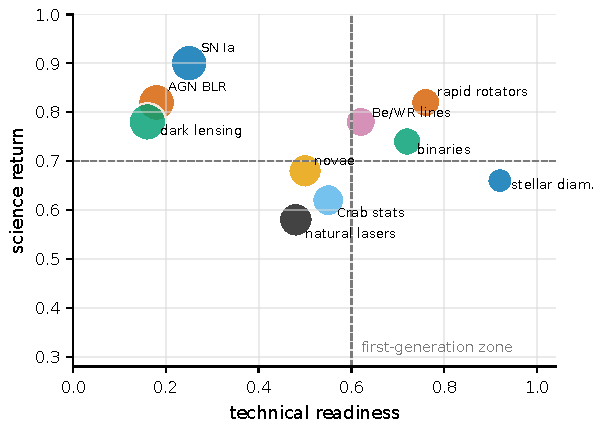
\includegraphics[width=0.78\linewidth]{figures/generated/chapter_19/ch19_priority_matrix.pdf}
\caption{The first-generation science-case matrix. The horizontal axis is technical maturity, the vertical axis is science return, and the larger the point, the higher the systematic-error and trigger risk. Targets in the upper right with smaller points are best suited as first-generation acceptance items; upper-left targets (Type Ia, AGN broad-line regions, dark-matter small-scale lensing) have high scientific value but need dedicated arrays or more mature quantum resources, and belong to the long-term category.}
\label{fig:e25-priority}
\end{figure}

The reading is this: targets in the \textbf{upper right with small points} (angular diameters of bright hot stars, reference stars of known diameter, \(\beta\) UMa-type A stars, MAGIC/VERITAS reproducible targets) are low-risk and reproducible, and naturally the first batch of acceptance projects; adding scientific information on the same capability are \(\gamma\) Cas-type rapid rotators, Be/WR line regions, close binaries, and early nova expansion; more dependent on event-table quality and time/spectral selection are Crab phase-resolved statistics and natural-laser candidate lines; while those high-value upper-left targets, such as Type Ia geometric distance, AGN broad-line regions, dark-matter small-scale lensing, and quantum-network-assisted imaging (Chapter \ref{chap:e24}), should be placed firmly among the long-term goals.

The table below lists side by side the first observable, typical order of magnitude, and ``whether it counts as first-generation'' criterion for the seven classes of case, for easy comparison. It is in fact the ranking of Eq.\ \eqref{eq:e25-priority-score} cashed out into an executable checklist:

\begin{longtable}{p{0.17\linewidth}p{0.22\linewidth}p{0.23\linewidth}p{0.20\linewidth}}
\toprule
Case & First observable & Typical order of magnitude & First-generation criterion \\
\midrule
Bright-star angular diameter & \(|V|^2(B)\) & \(m_V<5\), \(\theta=0.5\text{--}2\,\mathrm{mas}\) & Multi-night repeatable to \(3\text{--}5\%\) diameter precision. \\
Rapid rotation & Multi-position-angle \(|V|^2\) & Axial ratio \(1.1\text{--}1.5\), \(\theta<1\,\mathrm{mas}\) & Can distinguish disk from ellipse model. \\
Binary & \(|V|^2\) oscillation & Separation \(0.2\text{--}5\,\mathrm{mas}\), \(f>0.1\) & Has orbital prior, covers two or more position angles. \\
Be/WR line & Line/continuum \(|V|^2\) & \(\mathrm{H}\alpha\), He, Fe lines & Sufficient line flux, verifiable continuum subtraction. \\
Nova & \(\theta(t)\) & mas level after a few days & Fast trigger, can merge with line velocity. \\
Crab statistics & Phase-window \(g^{(2)}\), color correlation & \(P=33\,\mathrm{ms}\) & Ephemeris, background nebula, and absolute timing closed. \\
Natural laser & \(g^{(2)}\), line width, polarization & \(\Delta\nu\) narrow enough for high coherence time & Line separable from continuum, has null test. \\
Type Ia & \(|V|^2(\lambda,t)\) & \(m<12\), tens of \(\mu\mathrm{as}\) & Do after kilometer-scale array and fast trigger mature. \\
\bottomrule
\end{longtable}

The ordering changes dynamically with the state of the instrument, and this matters. When the system has just completed time synchronization and zero-baseline correlation calibration, bright-star angular diameters and reference-star reproduction are the most valuable; when six or more baselines can run stably and uv coverage improves, rapid rotation and binaries enter the main checklist; when narrowband filtering and high data throughput are reliable, natural lasers and line disks gain realistic room; and only when the array expands to kilometer scale and can respond quickly each year to nearby transients with \(m\lesssim12\) will Type Ia geometric distance rise to a front-line target \citep{2017MNRAS.472.4126G,2022MNRAS.512.1722K,2024MNRAS.529.4387A,2024ApJ...966...28A,2025ApJ...995..191A,2025PhRvD.111h3047K}. All these trade-offs must ultimately return to the error budget of Chapter \ref{chap:e15} to be reconciled line by line, and this is precisely what the next part on teaching and computational experiments (Chapter \ref{chap:e26}) will have you run through with your own hands.

\section*{Chapter Summary}
\addcontentsline{toc}{section}{Chapter Summary}

\begin{itemize}
  \item \textbf{Rank first, observe second.} Triage the cases with the three yardsticks of brightness, angular scale, and external prior, written as the ranking expression \eqref{eq:e25-priority-score}: science return, technical maturity, and prior add points, while systematic and trigger risk subtract them. The first generation should pick targets in the ``upper-right comfortable region'' and not be led by the nose by a pretty topic.
  \item \textbf{Angular diameter is the most mature first-generation product.} Through the uniform-disk/limb-darkening model it enters the effective-temperature equation \eqref{eq:e25-teff} directly, and \(T_{\rm eff}\propto\theta^{-1/2}\) makes a \(4\%\) diameter error propagate into only a \(2\%\) temperature error. VERITAS and MAGIC are already producing data in batches.
  \item \textbf{From ``how big'' to ``what shape.''} Rapid rotators require the elliptical-visibility equation \eqref{eq:e25-elliptical-visibility}, and must cover multiple position angles to pin down the axial ratio and position angle; \(\gamma\) Cas has been measured to be near critical rotation.
  \item \textbf{Binaries and line disks are resolved by the baseline.} A binary's \(|V|^2\) oscillates per Eq.\ \eqref{eq:e25-binary-visibility}, with amplitude \(2f/(1+f)^2\) shrinking rapidly with the flux ratio; line and continuum mix by flux weighting (Eq.\ \eqref{eq:e25-line-continuum}), and must be separated before being interpreted.
  \item \textbf{Expanding transients sort near from far.} The angular-expansion equation \eqref{eq:e25-expansion} gives the expansion parallax: a Galactic nova reaches mas within a few days and is a realistic target; a Type Ia at \(10\,\mathrm{Mpc}\) is only tens of \(\mu\mathrm{as}\), a long-term goal needing kilometer-scale arrays.
  \item \textbf{Photon statistics test ``non-thermal.''} The Crab uses the phase-window equation \eqref{eq:e25-pulse-phase} for phase-resolved \(g^{(2)}\); natural lasers use the multimode relation \eqref{eq:e25-mode-bunching} plus line width for a null test, because multimode thermal light disguises itself as coherent light.
  \item \textbf{The order shifts as the instrument matures.} From zero-baseline calibration, to multiple baselines, to narrowband high throughput, to kilometer-scale fast response, the roadmap is dynamic, and all ultimately return to the error budget of Chapter \ref{chap:e15} to be reconciled line by line.
\end{itemize}

\medskip
\noindent\textbf{Questions to Ponder}
\begin{itemize}
  \item If a bright star's angular diameter is measured to \(3\%\) precision, and the bolometric flux \(F_{\rm bol}\) also has an independent error of \(3\%\), use Eq.\ \eqref{eq:e25-teff} to estimate roughly the relative error of the effective temperature \(T_{\rm eff}\). (Hint: first find the logarithmic sensitivities of \(T\) to \(\theta\) and to \(F\) separately, then add them in quadrature as independent errors.)
  \item For a binary with flux ratio \(f=0.05\), use Eq.\ \eqref{eq:e25-binary-visibility} to compute the cosine amplitude of its \(|V|^2\) oscillation. To measure it within \(1\) hour, what does it demand of the photon-pair count and the system calibration (recall Chapter \ref{chap:e15})?
  \item Why is ``seeing a bright, narrow spectral line'' still insufficient to declare it a natural laser? What role does \(M\) in Eq.\ \eqref{eq:e25-mode-bunching} play in this judgment, and what null test would you design to rule out ``multimode thermal light in disguise''?
\end{itemize}
